\chapter{Modelado de configuración automática de infraestructuras distribuidas}
\label{cap:modelado}

[Revisar]\\

La extensión a la herramienta de configuración Puppet se ha hecho mediante el uso de tipos y proveedores personalizados. Mediante la definición de un nuevo tipo estamos añadiendo un nuevo recurso que Puppet puede administrar; para que Puppet sepa cómo administrar ese nuevo recurso debemos proporcionar un proveedor en el que se le indique lo que tiene que hacer.


\section{Modelado de recursos distribuidos: el recurso \emph{cloud}}

En Puppet, la definición clásica de recursos se presupone dentro del ámbito local del nodo. Es decir, para cada nodo especificamos qué recursos debe contener y cuál debe ser su estado. Sin embargo, el modelado de un recurso distribuido plantea ciertos desafíos al modelo anterior, ya que dicho modelo no está pensado teniendo en cuenta la problemática asociada a los sistemas distribuidos. \\

%En Puppet, la definición clásica de recursos se presupone dentro del ámbito local del nodo. Es decir, para cada nodo especificamos qué recursos debe contener. Sin embargo, el modelado de un recurso distribuido plantea ciertos desafíos al modelo anterior: se puede pensar que para modelar un recurso distribuido basta con que Puppet envíe a cada nodo la configuración necesaria para garantizar el comportamiento deseado, pero, ¿qué pasa cuando ese nodo falla? Si no hacemos nada, el recurso dejará de mantenerse en el estado deseado. Por lo tanto, a la hora de administrar un recurso distribuido hay que asegurarse de que los nodos están operativos y cumpliendo con su función. Asimismo, un recurso distribuido puede presentar elementos comunes con otros recursos distribuidos, tales como una monitorización básica. Entre los recursos clásicos de Puppet, por ejemplo un usuario y un paquete, no hay tantos elementos comunes. \\

Al modelar un recurso distribuido, deben tenerse en cuenta las características propias de este tipo de recursos. Tenemos que presentar el recurso como un único sistema coherente, es decir, como una única abstracción; no vale con modelar un recurso distribuido como una colección de recursos clásicos de Puppet. Afortunadamente Puppet proporciona los medios para crear nuevos tipos de recurso, y se puede crear un nuevo tipo de recurso con sus parámetros correspondientes para modelar los recursos distribuidos. \\

%%% Revisar [Metaclases]
% Tenemos, pues, dos tipos de recursos claramente diferenciados: los recursos clásicos de Puppet (a los que llamaremos recursos locales) y los recursos distribuidos. Para entender mejor el modelado de estos recursos se puede hacer una analogía con la programación orientada a objetos (Figura \ref{figure:puppet-modelo-teorico}). En esta analogía el recurso distribuido sería una instancia de una metaclase que proporcionaría los atributos y métodos comunes a todo recurso distribuido. La instanciación de ese recurso en un recurso distribuido de tipo AppScale, Torque, web u otros sería similar a la instanciación de una clase a partir de la metaclase. De igual manera, el recurso distribuido instanciado podría añadir nuevos atributos y métodos y modificar el comportamiento de los métodos de la metaclase, ya que no tienen por qué iniciarse de igual manera el recurso AppScale y el recurso Torque. Los recursos locales de Puppet quedarían como clases que se instanciarían a partir de una metaclase de recursos locales.

%\begin{figure} [!htbp]
%  \centering
%  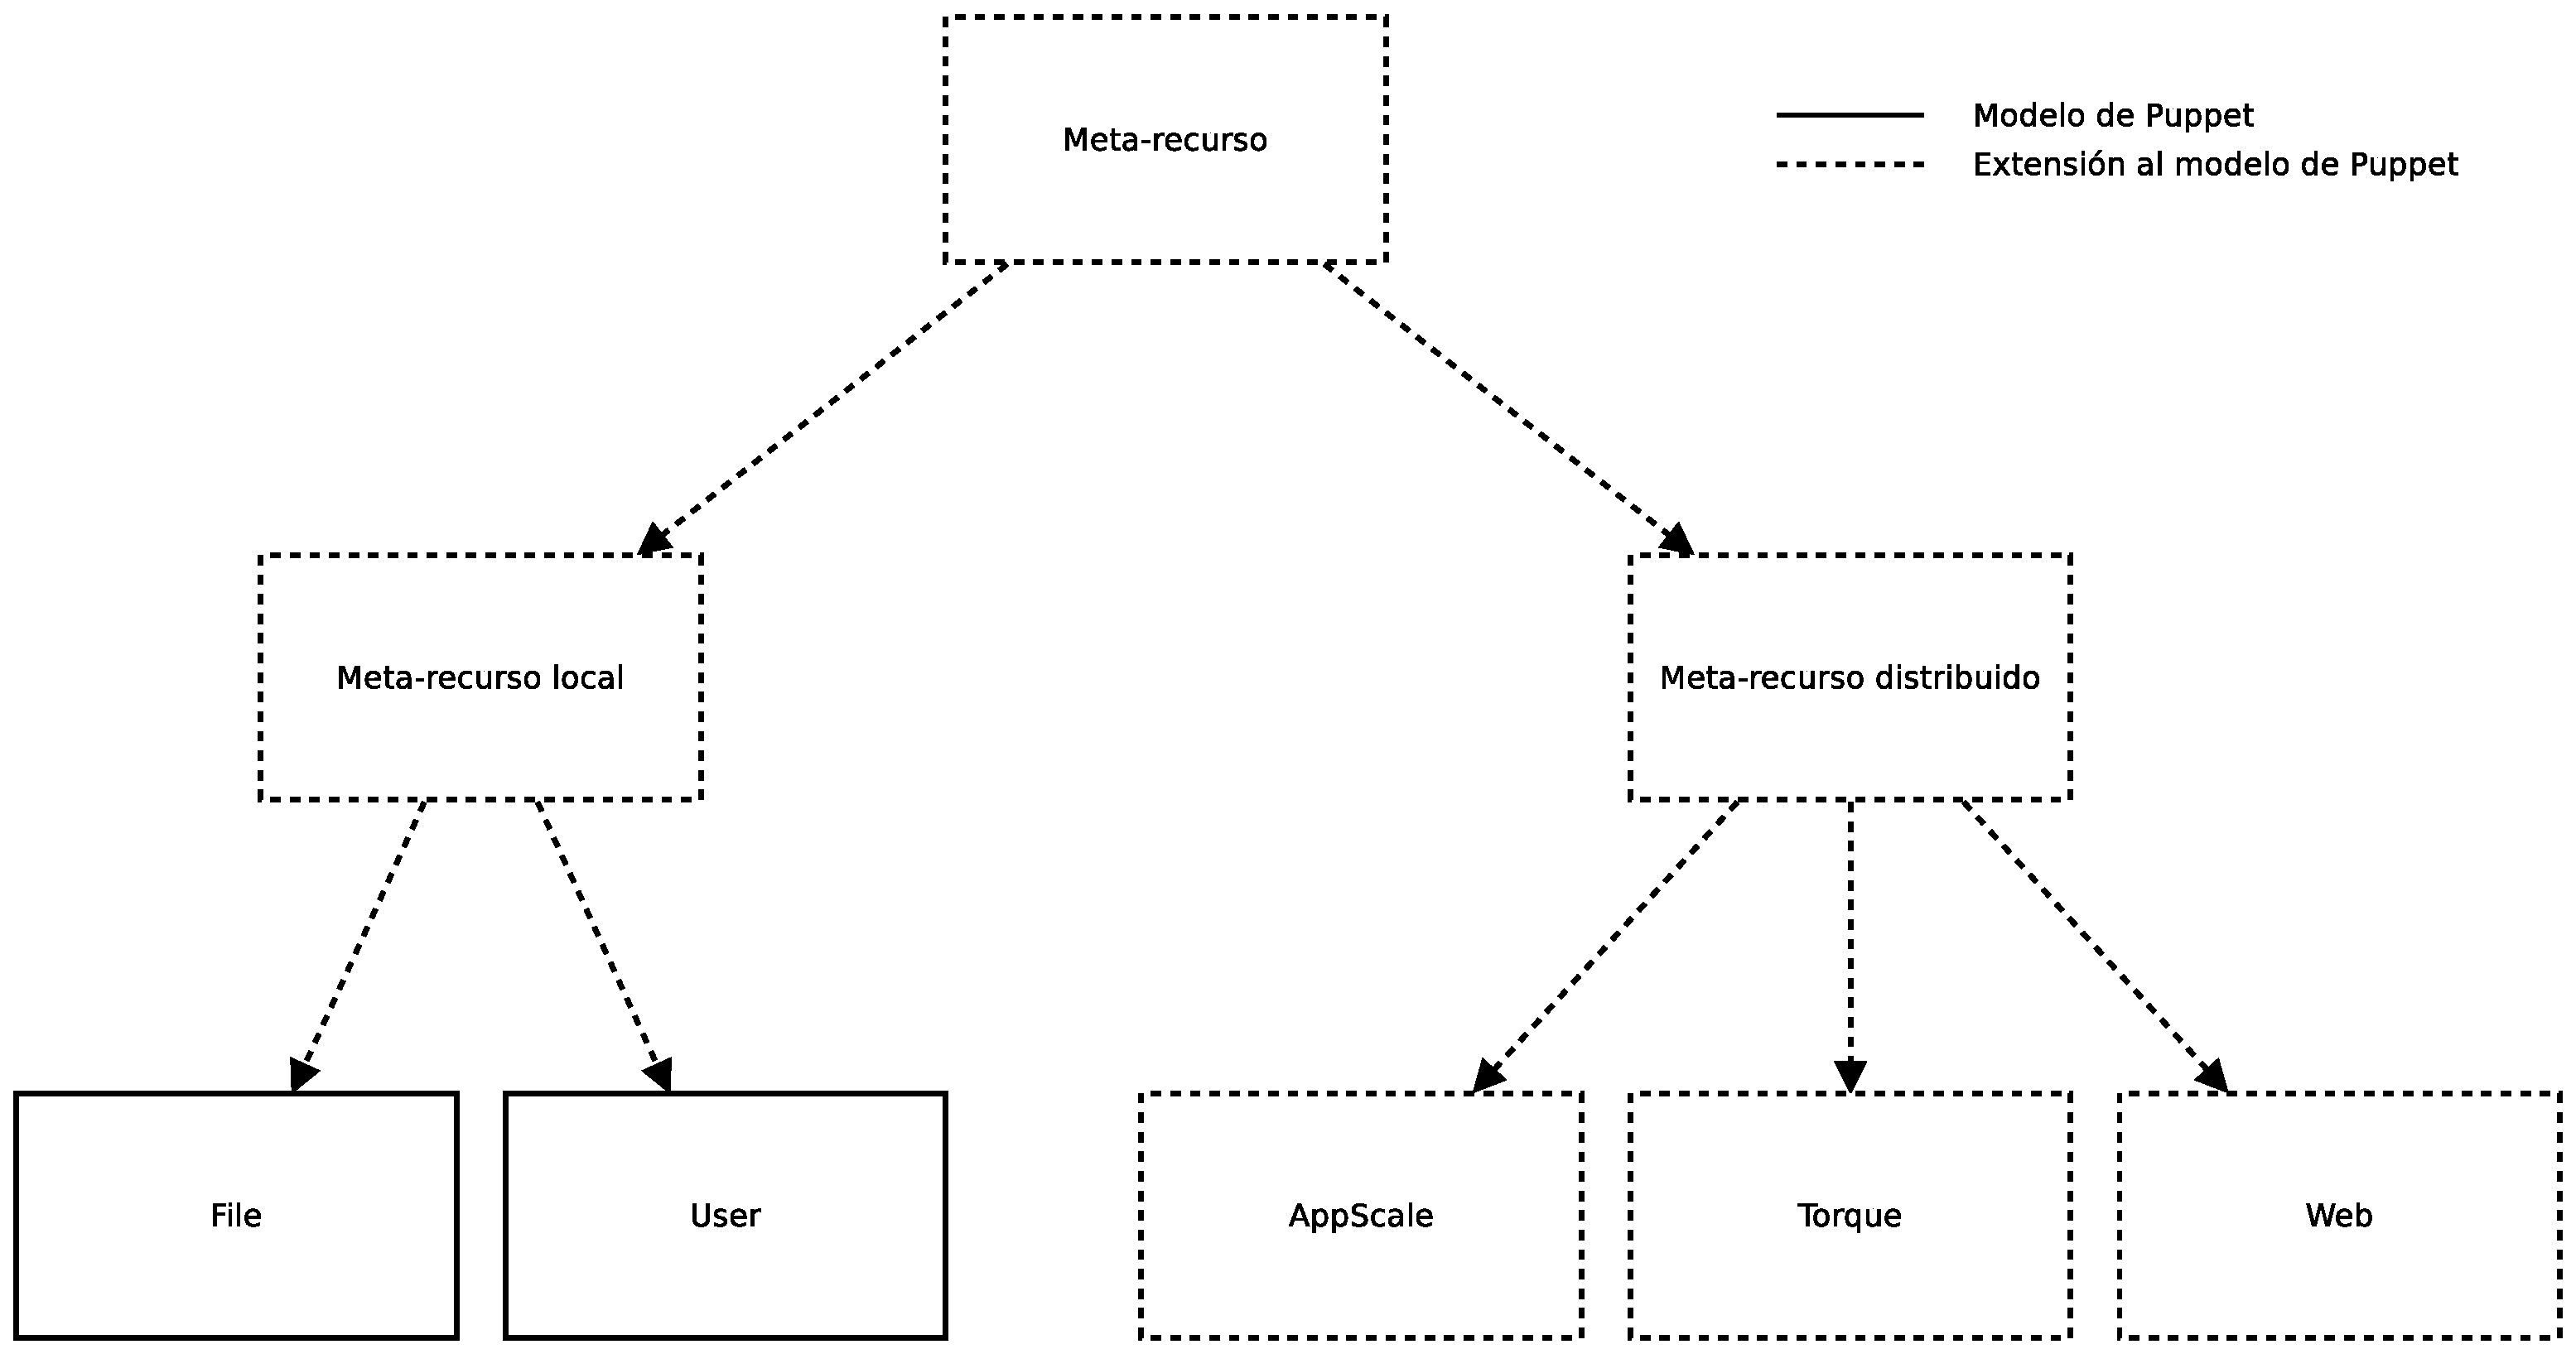
\includegraphics[width=\textwidth]{figuras/Modelo_Teorico_Puppet.eps}
%  \caption{Modelado teórico de recursos en Puppet.}
%\label{figure:puppet-modelo-teorico}
%\end{figure}

En particular, para modelar un distribuido, o recurso \emph{cloud}, se han considerado como fundamentales los siguientes parámetros:

\begin{itemize}
\item Nombre: Para identificar al \emph{cloud} de manera única.
\item Fichero de direcciones IP: Para describir qué dirección IP está asociada a cada nodo del \emph{cloud}. Como la asociación viene dada por un par <rol, dirección IP> también se le llama a este parámetro fichero de roles.
\item Fichero de imágenes de disco: Para asignar a cada nodo la correspondiente imagen de disco duro.
\item Fichero de dominio: Para definir una máquina virtual especificando sus características \emph{hardware}.
\item Conjunto de máquinas físicas: Para indicar qué máquinas físicas pueden ejecutar las máquinas virtuales definidas.
\end{itemize}

Si aplicamos este modelo a un recurso \emph{cloud} de tipo Torque podríamos hacerlo usando algo similar a:

\begin{lstlisting}
torque {'torque-cloud':
   ip_file  => "/etc/puppet/modules/torque/files/jobs-ip.yaml",
   img_file => "/etc/puppet/modules/torque/files/jobs-img.yaml",
   domain   => "/etc/puppet/modules/torque/files/mycloud-template.xml",
   pool     => ["155.210.155.70"],
   ensure   => running,
}
\end{lstlisting}


\section{Diseño del proveedor de recursos distribuidos}

Puppet puede ser extendido para incluir la definición de nuevos recursos. Para ello hay que proporcinarle, como mínimo, dos ficheros: uno en el que se define el recurso y otro en el que se define cómo gestionar ese recurso. Al fichero en el que se define el recurso se le llama tipo y al fichero en el que se define cómo gestionarlo se le llama proveedor. Es decir, el tipo se encarga del ``qué'' y el proveedor se encarga del ``cómo''.\\

En un recurso \emph{cloud} la definición en el fichero tipo contendría los parámetros propios de ese tipo de cloud. En el ejemplo anterior éstos serían: \texttt{ip\_file}, \texttt{img\_file}, \texttt{domain} y \texttt{pool} (el parámetro \texttt{ensure} es común a todo recurso puppet y se define automáticamente). Una vez modelado el recurso \emph{cloud}, queda como tarea proporcionar un proveedor que se encargue de llevar el \emph{cloud} al estado que se le indique desde el manifiesto Puppet.\\

Ahora bien, este proveedor no es un proveedor al uso: debe lidiar con la problemática asociada a los sistemas distribuidos. Entre otras cosas debe tener en cuenta que puede haber dependencias entre los nodos, que cada nodo puede cumplir un papel distinto dentro del sistema y que los nodos pueden fallar. Además, debe resolver los fallos con la mayor transparencia posible, es decir, con la menor intervención humana posible.\\

Para poner un \emph{cloud} en funcionamiento, los pasos que realiza el proveedor son:

\begin{itemize}
\item Comprobación de la existencia del \emph{cloud}: si existe se realizarán tareas de mantenimiento, si no existe se creará.
\item Comprobación del estado del conjunto de máquinas físicas.
\item Obtención de las direcciones IP de los nodos y los roles que les han sido asignados.
\item Comprobación del estado de las máquinas virtuales: si están funcionando se monitorizan, mientras que si no están funcionando hay que definir una nueva máquina virtual y ponerla en funcionamiento. Las funciones de monitorización incluyen el envío de un fichero mediante el cual cada nodo se autoadministre la mayor parte posible.
\item Cuando todas las máquinas virtuales estén funcionando se procede a inicializar el \emph{cloud}.
\item Operaciones de puesta en marcha particulares dependiendo de cada tipo de \emph{cloud}.
\end{itemize}

Una parte muy importante para el proveedor a la hora de poner en marcha, o mantener un \emph{cloud} es el parámetro \texttt{ip\_file}. En el fichero indicado por este parámetro se define una asociación entre la dirección IP del nodo y el rol que cumplirá ese nodo dentro del \emph{cloud}. Siguiendo con el ejemplo del recurso \emph{cloud} de tipo Torque, el fichero de roles en el que se especifica quién es el nodo maestro y la lista de nodos de computación sería similar a éste:

\begin{yamlcode}
--- 
:head: 155.210.155.73
:compute:
- 155.210.155.177
\end{yamlcode}

Para parar un \emph{cloud} los pasos que el proveedor realiza son:

\begin{itemize}
\item Comprobación de la existencia del \emph{cloud}: si existe se procederá a su parada.
\item Operaciones de parada particulares a cada tipo de \emph{cloud}.
\item Apagado y borrado de las definiciones de las máquinas virtuales creadas explícitamente para este \emph{cloud}.
\item Parada de las funciones de automantenimiento de los nodos.
\item Eliminación de los ficheros internos de gestión del \emph{cloud}.
\end{itemize}

La creación de un tipo y un proveedor no fue la primera opción que se barajó para realizar el modelado del recurso distribuido, sino que fue la de usar la API \emph{Faces} de Puppet. \emph{Faces} es una API para crear subcomandos y acciones dentro de Puppet. Después de analizar esta API a fondo se vio que las opciones que ofrecía no permitían la integración del recurso distribuido dentro del modelo de Puppet. Como lo que interesaba era crear una abstracción del recurso distribuido esta opción se acabó descartando en favor de la creación de un tipo y un proveedor, que soluciona el problema de una manera más elegante.
